% coding:utf-8

%----------------------------------------
%FOSAPHY, a LaTeX-Code for a summary of basic physics
%Copyright (C) 2013, Mario Felder

%This program is free software; you can redistribute it and/or
%modify it under the terms of the GNU General Public License
%as published by the Free Software Foundation; either version 2
%of the License, or (at your option) any later version.

%This program is distributed in the hope that it will be useful,
%but WITHOUT ANY WARRANTY; without even the implied warranty of
%MERCHANTABILITY or FITNESS FOR A PARTICULAR PURPOSE.  See the
%GNU General Public License for more details.
%----------------------------------------

\chapter{Zustandsraum}
\section{Regelungsnormalform der Zustandsgleichung}
\[
	G(s)= \frac{b_0+b_1s+b_2s^2+...+b_ns^n}{a_0+a_1s+a_2s^2+...+a_ns^n}
\]
\subsection{Regelungsnormalform}
\[
	\dot x=
	\underbrace{
		\begin{bmatrix}
			0 &	1 & 0 & .. & 0\\
			0 & 0 & 1 & .. & 0\\
			.. & .. & .. &.. & .. \\
			0 & 0 & 0 & .. & 1\\
			-\frac{a_0}{a_n} &-\frac{a_1}{a_n} & -\frac{a_2}{a_n} &.. &-\frac{a_{n-1}}{a_n}\\	
		\end{bmatrix}
	}_{\textbf{A}}
	\cdot x +
	\underbrace{
		\begin{bmatrix}
			0 \\
			0 \\
			.. \\
			0 \\
			\frac{1}{a_n} \\	
		\end{bmatrix}
	}_{\textbf{b}}
	\cdot u	
\]

\[
	y=
	\underbrace{
			\begin{bmatrix}
				b_0-a_0\frac{b_n}{a_n} & b_1-a_1\frac{b_n}{a_n} & .. & b_{n-1}-a_{n-1}\frac{b_n}{a_n} &\\
			\end{bmatrix}
	}_{\textbf{$c^T$}}
	\cdot x  +
	\underbrace{
		\left[ \frac{b_n}{a_n} \right] 
	}_{\textbf{d}}
	\cdot u
\]

\subsection{Beobachtungsnormalform}
\[
	\dot x=
	\underbrace{
		\begin{bmatrix}
			0 &	0 & 0 & .. & -\frac{a_0}{a_n}\\
			1 & 0 & 0 & .. & -\frac{a_1}{a_n}\\
			0 & 1 & 0 & .. & -\frac{a_2}{a_n}\\
			.. & .. & .. &.. & .. \\
			0 & 0 & .. & 1 &-\frac{a_{n-1}}{a_n}\\	
		\end{bmatrix}
	}_{\textbf{A}}
	\cdot x +
	\underbrace{
		\begin{bmatrix}
			b_0-b_n\frac{a_0}{a_n} \\
			b_1-b_n\frac{a_1}{a_n} \\
			b_2-b_n\frac{a_2}{a_n}  \\
			..\\
			b_{n-1}-b_n\frac{a_{n-1}}{a_n}\\	
		\end{bmatrix}
	}_{\textbf{b}}
	\cdot u	
\]
\[
	y=
	\underbrace{
			\begin{bmatrix}
				0 & 0 & .. & 0 & \frac{1}{a_n}\\
			\end{bmatrix}
	}_{\textbf{$c^T$}}
	\cdot x  +
	\underbrace{
		\left[ \frac{b_n}{a_n} \right] 
	}_{\textbf{d}}
	\cdot u
\]
\subsection{Jordanische Normalform}
\begin{itemize}
      \item Bevorzugte Verwendung, wenn Pole vom System bekannt sind
      \item System ist vollständig entkoppelt, wenn alle Pole reell und einfach vorkommen
      \item A ist Diagonalmatrix mit $\lambda_i$: Pole
\end{itemize}

\[
	\dot x=
	\underbrace{
		\begin{bmatrix}
			\lambda_1 &	0 & 0 & .. & 0\\
			0 & \lambda_2 & 0 & .. & 0\\
			0 & 0 & \lambda_2 & .. & 0\\
			.. & .. & .. &.. & .. \\
			0 & 0 & 0 & .. & \lambda_n\\	
		\end{bmatrix}
	}_{\textbf{A}}
	\cdot x +
	\underbrace{
		\begin{bmatrix}
			1 \\
			1 \\
			.. \\
			.. \\
			1\\	
		\end{bmatrix}
	}_{\textbf{b}}
	\cdot u	
\]

\[
	y=
	\underbrace{
			\begin{bmatrix}
				r_1 & r_2 & .. & r_n\\
			\end{bmatrix}
	}_{\textbf{$c^T$}}
	\cdot x  +
	\underbrace{
		\left[ r_0 \right] 
	}_{\textbf{d}}
	\cdot u
\]
\section{Steuerbarkeit und Beobachtbarkeit}
\subsection{Steuerbarkeit}
Das System heisst steuerbar, wenn sein Zustandspunkt \underline{x} durch geeignete Wahl des Steuervektors u in endlicher Zeit aus einem beliebigen Anfangszustand $x_0$ in den Endzustnad 0 bewegt werden kann (Steuerbar wenn die Vektoren linear unabhängig sind; $Rang(Q_s) = n$ oder $det(Q_s)\neq 0$)
\[
	Q_s = 
	\begin{bmatrix}
			b	&	A\cdot b	& .. & A^{n-1} \cdot b\\
	\end{bmatrix}
	= \left[ n \cdot n\right] 
\]
\subsection{Beobachtbarkeit}
Das System heisst beobachtbar, wenn dem bekannten $u(t)$ aus der Messung $y(t)$ über eine endliche Zeitspanne der Anfangszustand $x(t)$ eindeutig ermittelt werden kann, ganz gleich wo dieser liegt.\\
\\
Das System ist beobachtbar, wenn die Beobachtungsmatrix $Q_B$ regulär ist (nxn Matrix) ($det(Q_B)\neq 0$).
\[
	Q_B=
	\begin{bmatrix}
		c^T\\
		c^T \cdot A\\
		...\\
		c^T\cdot A^{n-1}\\
	\end{bmatrix}
\]
\section{Transformation}
\subsection{Transformation in Regelungsnormalform (Steuernormalform)}
Eine Übertragungssystem $\dot{x}=A\cdot x +  b \cdot u$ wird mit der Transformation $z=T_R\cdot x$ in die Regelungsnormalform  $\dot{x_R}=A_R\cdot x_R +  b_R \cdot u$ überführt.\\
\\
$q_{s_n}^T$ ist die letzte Zeile von der inversen Steuerbarkeitsmatrix $Q_s^{-1}$.
\[
	A_R = T_R\cdot A \cdot T_R^{-1}	\\	b_R = T_R\cdot b	\\	c_R^T = c^T\cdot T_R^{-1}	\\	d_R = d
\]
\[
	T_R=
	\begin{bmatrix}
		q_{s_n}^T \\
		q_{s_n}^T \cdot A \\
		.. \\
		q_{s_n}^T \cdot A^{n-1}\\	
	\end{bmatrix}	\\
	Q_s^{-1} =
	\begin{bmatrix}
			.. &	.. & .. & .. & ..\\
			.. &	.. & .. & .. & ..\\
			.. &	.. & .. & .. & ..\\
			 [x &	x & x & x & x]  \\	 
	\end{bmatrix}
\]

\subsection{Transformation auf Beobachtungsnormalform}
Eine Übertragungssystem $\dot{x}=A\cdot x +  b \cdot u$ wird mit der Transformation  $z=T_B\cdot x$ in die Beobachtungsnormalform $\dot{x_B}=A_R\cdot x_B +  b_B \cdot u$ überführt.\\
\\
$q_{B_n}$ ist die letzte Spalte von der inversen Beobachtungsmatrix $Q_B^{-1}$.
\\
\[
	A_B = T_B\cdot A \cdot T_B^{-1}	\\	b_B = T_B\cdot b	\\	c_B^T = c^T\cdot T_B^{-1}	\\	d_B = d
\]
\\
\[
	T_B=
	\begin{bmatrix}
		q_{B_n} & A\cdot q_{B_n} &  ..& A^{n-1}\cdot q_{B_n} & \\
	\end{bmatrix}	\\
	Q_B^{-1} =
	\begin{bmatrix}
			 .. & .. & x\\
			 .. & .. & x\\
			 .. & .. & x\\	 
	\end{bmatrix}
\]

\section{Reglersynthese im Zustandsraum}
\begin{center}
	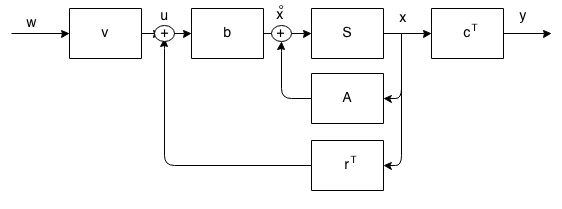
\includegraphics[scale = 0.4]{images/zustandsregler.png}
\end{center}
\[
	A_{CL}= A-b\cdot r^T	\\ A_R=T_R\cdot A \cdot T_R^{-1}
\]
\[
	A_{R,CL}= A_R-b_R\cdot r_R^T	\\	r_R^T=
		\begin{bmatrix}
				r_{1,R}	&	r_{2,R}	& r_{3,R} &r_{n,R}\\
		\end{bmatrix}
\]
Daraus folgt:
\[
		A_{Cl,R}=
		\begin{bmatrix}
			0 &	1 & 0 & .. & 0\\
			0 & 0 & 1 & .. & 0\\
			.. & .. & .. &.. & .. \\
			0 & 0 & 0 & .. & 1\\
				\underbrace{
					-\frac{a_0}{a_n}-r_{1,R} 
				}_{\textbf{$-c^{n-1}$}}
		 &-\frac{a_1}{a_n}-r_{2,R} & -\frac{a_2}{a_n}-r_{3,R} &.. &-\frac{a_{n-1}}{a_n}-r_{n,R}\\	
		\end{bmatrix}
\]
Diese Matrix kann gerade in das Istpolynom überführt werden.
\\
Istpolynom:
\[
	p_{Cl,r}(s)=s^n+
	\underbrace{(a_{n-1}+r_{n,R})	}_{\textbf{$c^{n-1}$}}
	\cdot s^{n-1}+...+(a_{1}+r_{2,R})a_1\cdot s +(a_0+r_{1,r})
\]
Das Sollpolynom ist durch die Nullstellen vorgegeben:
\[
	p(s)=s^n+p_{n-1}\cdot s^{n-1}+...+p_1\cdot s +p_0
\]
Koeffizientenvergleich ergibt nun:
\[
	r_{1,R}=p_0-a_0
\]
\[
	r_{2,R}=p_1-a_1
\]
\[
	r_{n,R}=p_{n-1}-a_{n-1}
\]
\\
\\
Durch die Transformation in RNF der letzten Zeile von $Q_s^{-1}$ (T) lässt sich die Matrix umwandeln.
\[
	r^T=r_R^T \cdot T
\]


\subsection{Vorfilter / Vorverstärker}
Der Vorfilter/Vorverstärker gewährleistet, dass im stationärem Zustand y mit dem gewünschtem, konstantem Vektor w übereinstimmt.
\[
	 	v=[c^T(b\cdot r^T-A)^{-1}\cdot b]^{-1}
\]
\\
\subsection{Beobachter}
Beobachter ist ein Nachbau des System für den Rechner. Er beinhaltet alle Punkte des realen System. Dafür werden keine Sensoren benötigt. Die Variablen werden geschätzt.\\
\\
Das $h$ muss derart bestimmt werden, dass $eigW(A-h_c^T)<0$ sind.\\
\\
Falls das System in BNF vorliegt, gilt:
\[
	A_B=T_B^{-1}\cdot A \cdot T_b	\\	c_B^T=c^T\cdot T_B = [0 \ 0 \ .. \  1]	\\	b_B=T_B^{-1}\cdot b
\]
\[
	A_B= \begin{bmatrix}
				0 &	0 & 0 & .. & -\frac{a_0}{a_n}\\
				1 & 0 & 0 & .. & -\frac{a_1}{a_n}\\
				0 & 1 & 0 & .. & -\frac{a_2}{a_n}\\
				.. & .. & .. &.. & .. \\
				0 & 0 & .. & 1 &-\frac{a_{n-1}}{a_n}\\	
			\end{bmatrix}
\]
Folgende Gleichung wird für die Bestimmung des Istpolynoms benötigt. Da $a_n=1$, kann folgende Vereinfachung gemacht werden:
\[
	\dot{e}_{x,B}=(A_B-h_B\cdot c_B^T)\cdot e_{x,B}=
	\begin{bmatrix}
					0 &	0 & 0 & .. & -a_0-h_{B,1}\\
					1 & 0 & 0 & .. & -a_1-h_{B,2}\\
					0 & 1 & 0 & .. & -a_2-h_{B,3}\\
					.. & .. & .. &.. & .. \\
					0 & 0 & .. & 1 &-a_{n-1}-h_{B,n}\\	
				\end{bmatrix}
\]

Istpolynom:
\[
	u(s)=s^n+(a_{n-1}+h_{B,n})s^{n-1}+...+(a_1+h_{B,2})s+(a_0+h_{B,1})
\]
Sollpolynom:
\[
	p(s)=s^n+p_{n-1}s^{n-1}+...+p_1 s+p_0
\]
Aus diesen beiden Gleichungen kann via Koeffizientenvergleich die Matrix $h_B$ bestimmt werden.
\[
	h_{B,1}=p_0-a_0	\\	h_{B,2}=p1-a1	\\	etc.	
\]
\[
	h_B=p-a
\]